
\chapter{Sprint 1 : Création du dataset et mise en place du pipeline OCR}
\label{chap:sprint1}

% Introducing Sprint 1
\section{Introduction}
\label{sec:intro_sprint1}

Ce chapitre décrit le Sprint 1, première itération du développement d’un système de collecte de données en temps réel et de gestion des alertes pour les appareils médicaux en salle de réveil, comme présenté dans l’introduction générale et d’étude architecturale. Selon la planification établie dans le chapitre précédent, cette phase se concentre sur la création d’un dataset annoté à partir de moniteurs médicaux et sur le développement d’un pipeline OCR basé sur des technologies de détection et de reconnaissance de texte pour extraire les signes vitaux, tels que la fréquence cardiaque, la pression artérielle et la saturation en oxygène. Cette itération pose les bases techniques pour la collecte automatisée des données, un objectif central du projet, en suivant la méthodologie Scrum décrite dans le chapitre consacré à la méthode.

\begin{figure}[H]
    \centering
    \begin{tikzpicture}[
        node distance=1cm and 1.5cm,
        box/.style={
            rectangle, rounded corners, draw=black, thick, 
            fill=gray!15, minimum height=1.2cm, minimum width=2cm, align=center
        },
        arrow/.style={-Stealth, thick}
    ]
        % Nodes
        \node[box] (camera) {Caméras IP};
        \node[box, right=of camera] (flask) {Serveur Flask};
        \node[box, above right=1cm and 1.5cm of flask] (roboflow) {Roboflow API};
        \node[box, below right=1cm and 1.5cm of flask] (tesseract) {Tesseract OCR};
        \node[box, right=2cm of flask] (laravel) {Backend Laravel};
        \node[box, right=of laravel] (db) {Base de données};

        % Arrows
        \draw[arrow] (camera) -- (flask);
        \draw[arrow] (flask) -- (roboflow);
        \draw[arrow] (flask) -- (tesseract);
        \draw[arrow] (flask) -- (laravel);
        \draw[arrow] (laravel) -- (db);
    \end{tikzpicture}
    \caption{Architecture du système pour le Sprint 1}
    \label{fig:architecture_sprint1}
\end{figure}

% Defining objectives for Sprint 1
\section{Objectifs du Sprint 1}
\label{sec:objectifs_sprint1}

L’objectif principal du Sprint 1 est de développer un pipeline fonctionnel permettant la collecte en temps réel des données affichées sur les écrans des moniteurs à l’aide de caméras IP. Cette phase vise à créer un dataset annoté d’images des moniteurs, avec des annotations précises pour identifier les signes vitaux. Un modèle de détection YOLO est entraîné pour repérer les régions d’intérêt contenant ces données. Des outils de traitement d’image et de reconnaissance optique de caractères (OCR) avec Tesseract sont intégrés pour extraire les valeurs textuelles. Les caméras IP sont configurées pour garantir une capture stable et optimale des images. Une API REST, implémentée avec Flask, est développée pour permettre l’intégration du pipeline dans les phases suivantes, avec une documentation Swagger et une authentification par clé API. Ces objectifs s’alignent sur les tâches prioritaires du Product Backlog et les besoins fonctionnels d’interopérabilité avec différents moniteurs, comme détaillé dans le chapitre précédent.

% Defining Sprint Backlog
\subsection*{Sprint Backlog}
\label{subsec:sprint_backlog}

Le Sprint Backlog pour le Sprint 1 regroupe les tâches sélectionnées du Product Backlog (voir Tableau \ref{tab:backlog}) pour répondre aux objectifs de cette itération. Chaque tâche est associée à une priorité, une estimation de l’effort en heures, et des critères d’acceptation pour garantir la qualité des livrables. Les tâches incluent la configuration du matériel, la capture et l’annotation des images, l’entraînement du modèle de détection, et le développement du pipeline OCR avec une API REST.

\begin{table}[H]
\centering
\caption{Sprint Backlog}
\label{tab:sprint_backlog_sprint1}
\begin{tabular}{|p{1.5cm}|p{6cm}|p{1.5cm}|p{2cm}|p{3cm}|}
\hline
\textbf{ID} & \textbf{Tâche} & \textbf{Priorité} & \textbf{Effort (h)} & \textbf{Critères d’Acceptation} \\
\hline
M-01 & Détection et reconnaissance des valeurs vitales via YOLO et OCR pour les moniteurs. & M & 80 & Précision de détection > 90\%, OCR extrait les valeurs avec < 5\% d’erreurs, compatible avec 3 moniteurs différents. \\
\hline
M-06 & Stockage et historique des données dans une base de données. & M & 20 & Base de données relationnelle configurée, stockage des données extraites testé avec succès. \\
\hline
S-04 & Interface Swagger pour l’API REST. & M & 10 & Documentation de l’API générée, accessible via Swagger UI, toutes les routes documentées. \\ 
\hline
\end{tabular}
\end{table}

% Describing tasks completed in Sprint 1
\section{Tâches réalisées}
\label{sec:taches_sprint1}

Les tâches réalisées reflètent les engagements pris lors de la planification du Sprint 1 et sont organisées en sous-sections pour plus de clarté.

% Configuring hardware
\subsection{Configuration du matériel}
\label{subsec:config_materiel}

L’environnement matériel a été préparé pour répondre aux besoins du pipeline. Des caméras IP ont été configurées à l’aide d’une application mobile dédiée, offrant une interface intuitive pour ajuster la résolution et l’exposition. Un serveur local, équipé d’un système d’exploitation Linux avec accélération GPU, a été mis en place pour supporter l’entraînement du modèle YOLO et l’exécution du pipeline OCR. Les bibliothèques nécessaires, telles que OpenCV, Tesseract, et les dépendances Python, ont été installées via pip dans un environnement virtuel.

% Capturing and annotating images
\subsection{Capture et annotation des images}
\label{subsec:capture_annotation}

La création du dataset a débuté par la capture d’images des écrans des moniteurs médicaux à l’aide de caméras IP. Ces images ont été prises dans des conditions d’éclairage contrôlé pour minimiser les reflets. Les images ont été annotées à l’aide de la plateforme Roboflow, en traçant des régions d’intérêt autour des paramètres vitaux, tels que la fréquence cardiaque, la pression artérielle et la saturation en oxygène. Le dataset a été divisé en ensembles pour l’entraînement, la validation et les tests, suivant une répartition de 80 \% pour l’entraînement, 10 \% pour la validation et 10 \% pour les tests. Pour améliorer la robustesse du modèle, des techniques d’augmentation des données, telles que la rotation, le recadrage et l’ajustement de la luminosité, ont été appliquées via des filtres d’image sur Roboflow, augmentant ainsi la taille du dataset d’entraînement.

% Training the model's detection
\subsection{Entraînement du modèle de détection}
\label{subsec:entrainement_yolo}

Un modèle YOLO, choisi pour sa rapidité et sa précision, a été entraîné sur la plateforme Roboflow avec le dataset annoté. Les hyperparamètres, tels que le taux d’apprentissage et le nombre d’époques, ont été optimisés pour maximiser les performances. Le modèle a atteint une mAP@50 de 83,2 \% sur l’ensemble de validation, avec une précision globale de 84,9 \% et un rappel de 71,3 \%. Des techniques comme la non-maximum suppression (NMS) et l’ajustement du seuil de confiance ont réduit les fausses détections. Les performances par classe sont détaillées dans le Tableau \ref{tab:precision_classes_sprint1}.

\begin{table}[H]
\centering
\caption{Précision par classe pour le modèle de détection sur le jeu de validation}
\label{tab:precision_classes_sprint1}
\begin{tabular}{|l|c|}
\hline
\textbf{Classe} & \textbf{Précision (\%)} \\
\hline
Taux respiratoire d’éveil (AwRR) & 83,0 \\
Pression diastolique (DIA) & 75,0 \\
Électrocardiogramme (ECG) & 93,0 \\
Dioxyde de carbone de fin d’expiration (EtCO2) & 94,0 \\
Fréquence cardiaque (HR) & 81,0 \\
Pression artérielle moyenne (MAP) & 77,0 \\
Pouls (PR/PULSE) & 100,0 \\
Respiration (RESP) & 76,0 \\
Taux respiratoire (RR) & 37,0 \\
Pression systolique (SYS) & 90,0 \\
Saturation en oxygène (SpO2) & 94,0 \\
Température du sang (TBLOOD) & 100,0 \\
Température (TEMP) & 90,0 \\
\hline
\end{tabular}
\end{table}

Le processus d’entraînement est illustré dans la Figure \ref{fig:courbe_yolo}, montrant la courbe d’apprentissage du modèle avec une diminution progressive de la perte et une amélioration de la précision au fil des époques. Le modèle a été exporté et déployé sur Roboflow pour une utilisation ultérieure dans le pipeline OCR.
\begin{figure}[H]
\centering
\caption{Courbe d’apprentissage du modèle de détection}
\label{fig:courbe_yolo}
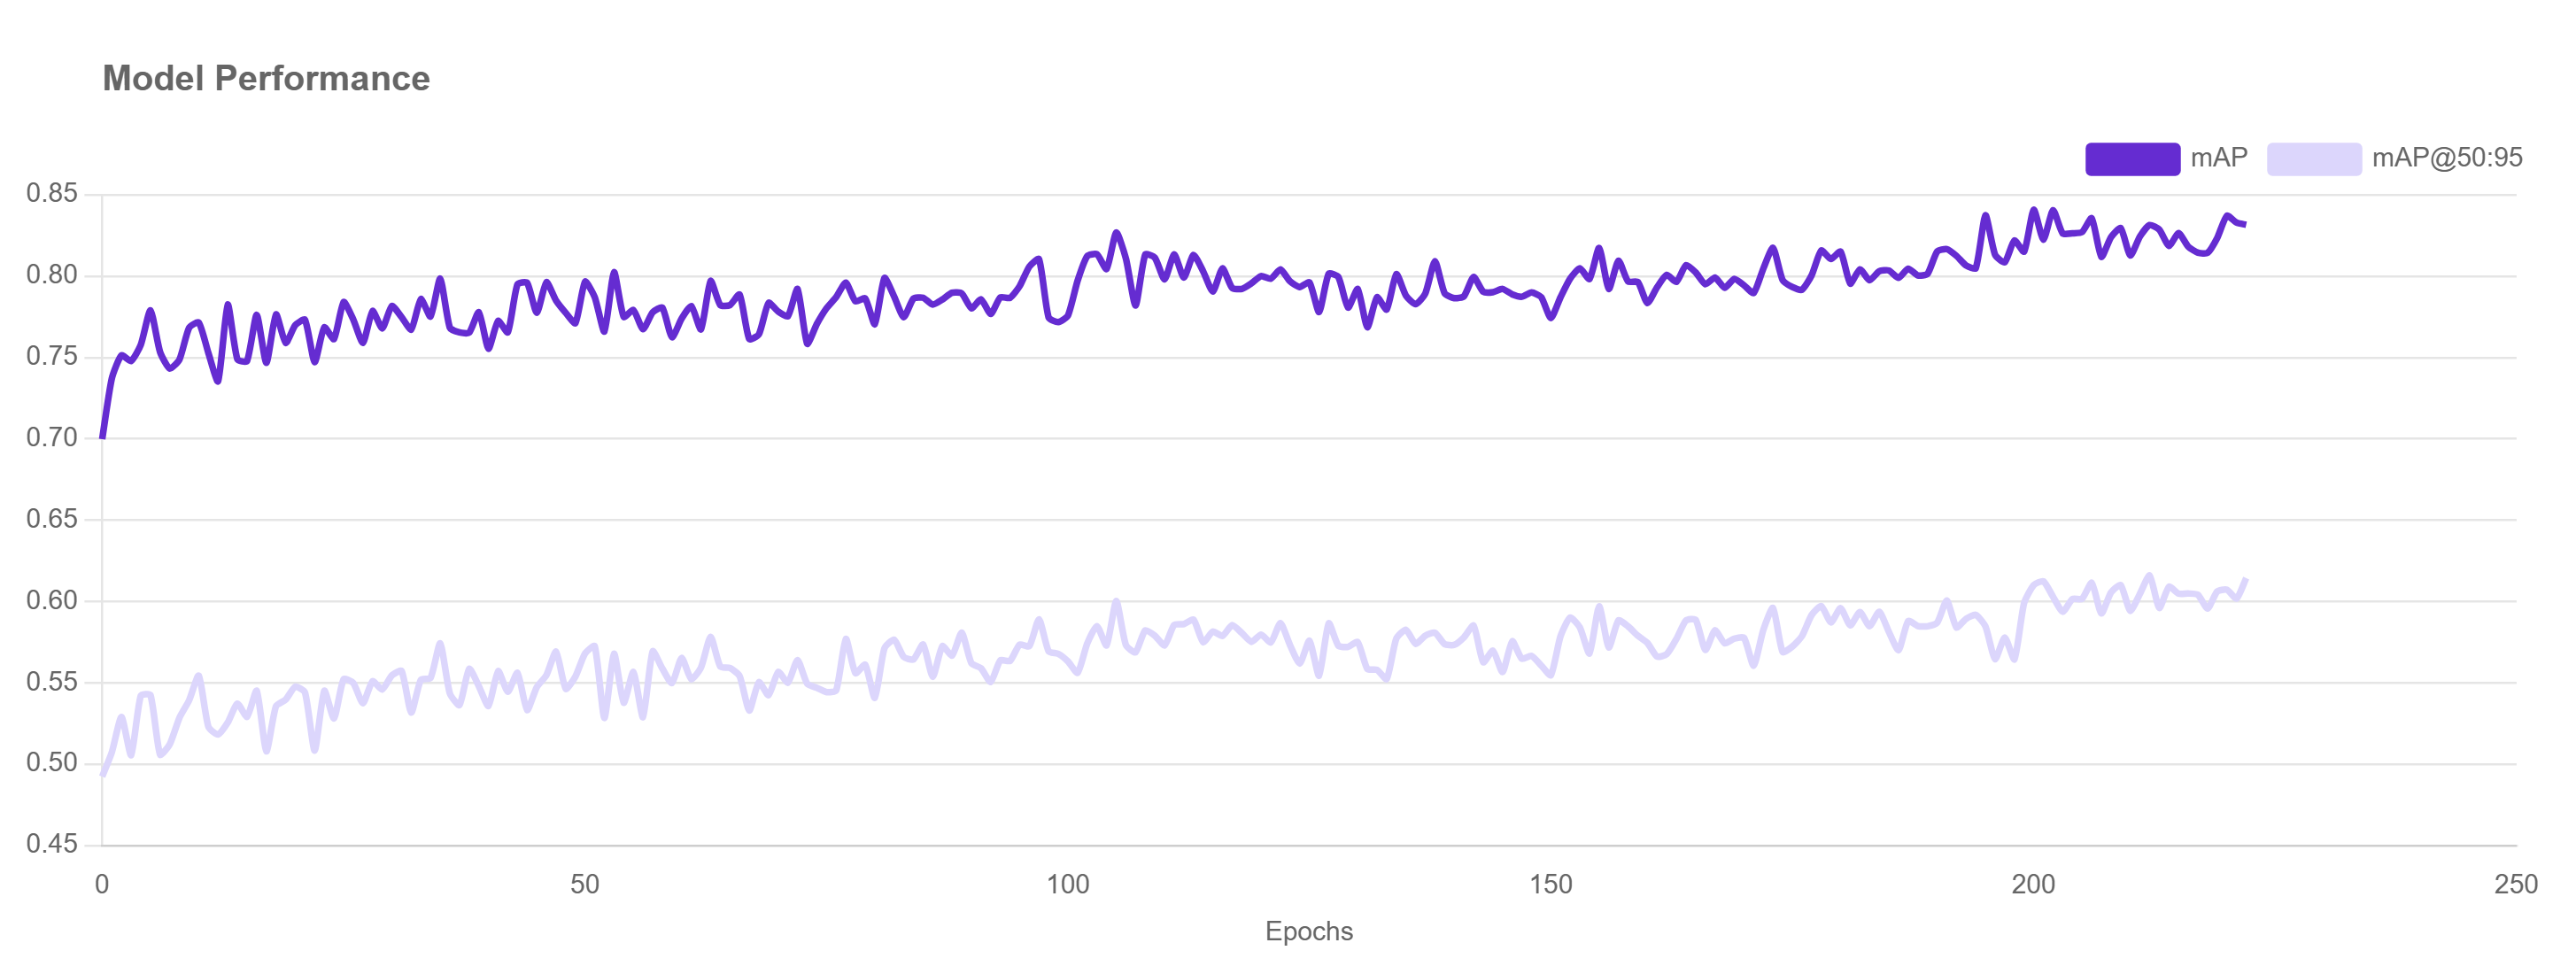
\includegraphics[width=0.8\textwidth]{chapter5/sections/diagrams/yolo_learning_curve.png}
\end{figure}

% Developing the OCR pipeline
\subsection{Développement du pipeline OCR}
\label{subsec:pipeline_ocr}

Le pipeline OCR a été développé sous forme d’une application Flask, permettant le traitement en temps réel des flux vidéo en provenance de caméras IP. Chaque flux est géré par un thread dédié, assurant ainsi la prise en charge simultanée de plusieurs caméras avec une synchronisation via un verrou pour éviter les conflits d’accès. Les images extraites sont prétraitées à l’aide d’OpenCV pour être converties en niveaux de gris, avec un renforcement du contraste et une réduction du bruit, améliorant la lisibilité pour l’OCR. Les régions d’intérêt (ROIs), identifiées à l’aide d’un modèle YOLO hébergé sur Roboflow, sont ensuite recadrées. Ces ROIs sont traitées par Tesseract OCR afin d’en extraire les valeurs numériques pertinentes. Des expressions régulières sont utilisées pour valider les formats des données extraites, permettant de rejeter les résultats non conformes. Une fois validées, les données sont envoyées vers un serveur Laravel via des requêtes HTTP POST. L’API REST développée expose plusieurs endpoints pour le contrôle des caméras (démarrage, arrêt, liste, statut), protégés par une authentification via clé API. Une documentation interactive est générée automatiquement à l’aide de Swagger UI, comme illustré dans la Figure \ref{fig:swagger_ui}. 

\begin{figure}[H]
    \centering
    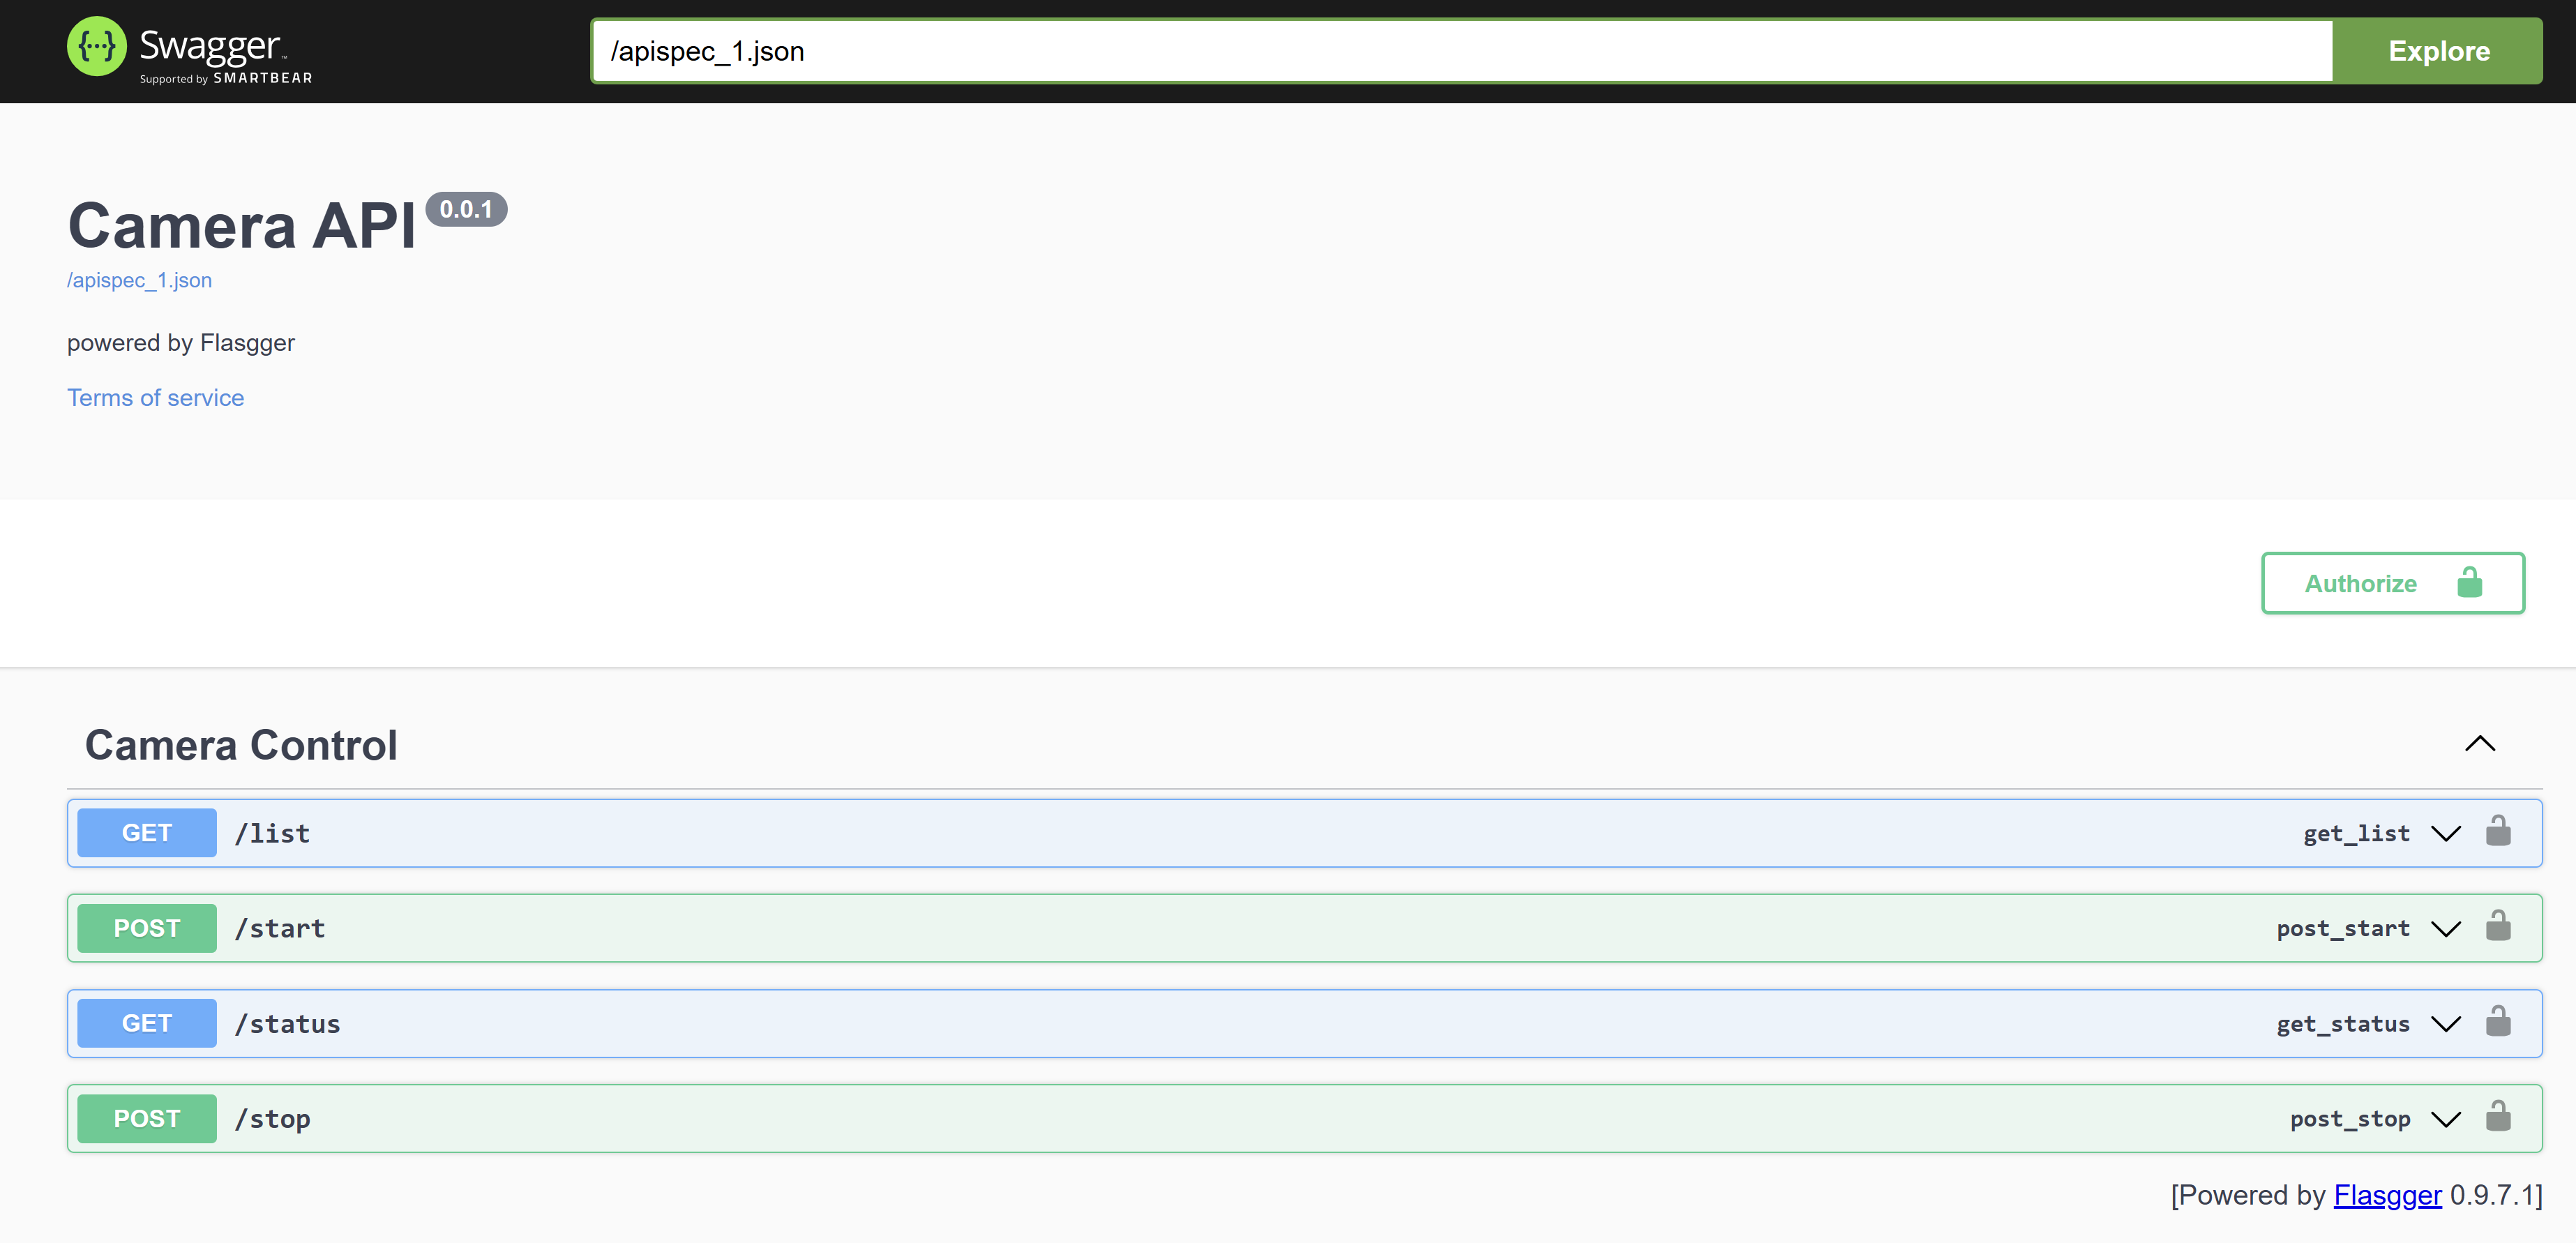
\includegraphics[width=0.8\textwidth]{chapter5/sections/images/swagger.png}
    \caption{Capture d’écran de l’interface Swagger UI pour la documentation de l’API REST}
    \label{fig:swagger_ui}
\end{figure}
% La Figure \ref{fig:sequence_workflow} présente le diagramme de séquence illustrant le workflow du pipeline OCR.
La Figure \ref{fig:sequence_workflow} présente le diagramme de séquence illustrant le workflow du pipeline OCR, montrant les interactions entre les caméras IP, le serveur Flask, le modèle YOLO, Tesseract OCR et le backend Laravel pour la collecte et le traitement des données.
\begin{figure}[H]
    \centering
    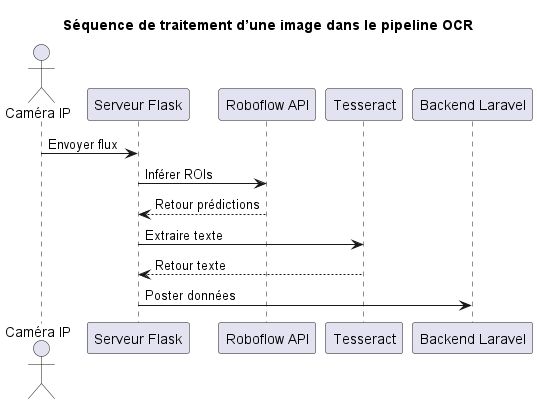
\includegraphics[width=0.8\textwidth]{chapter5/sections/diagrams/pipeline_workflow.png}
    \caption{Diagramme de séquence du workflow du pipeline OCR}
    \label{fig:sequence_workflow}
\end{figure}

% Testing integration and initial deployment
\subsection{Tests d’intégration et déploiement initial}
\label{subsec:integration_deployment}

Le pipeline a été testé sur un serveur Linux, avec Docker pour conteneuriser l’application Flask et ses dépendances. Les caméras IP ont été connectées au serveur via un réseau Wi-Fi sécurisé, avec un débit de 30 images par seconde. Le pipeline a été testé en conditions réelles, traitant des flux vidéo pour simuler la collecte en temps réel. Les tests ont validé une compatibilité avec trois modèles de moniteurs médicaux différents, avec des variations d’éclairage modérées. La latence moyenne du pipeline, mesurée à 150 ms par image, était conforme aux exigences. Le système a été intégré à un backend Laravel pour le stockage des données extraites dans une base de données relationnelle.

% Listing deliverables
\section{Livrables du Sprint 1}
\label{sec:livrables_sprint1}

Les livrables incluent :
\begin{itemize}
    \item Un dataset annoté, comprenant 10 000 images des moniteurs avec annotations, stocké sur un dépôt Roboflow.
    \item Un modèle YOLO entraîné, déployé sur le serveur Roboflow avec une mAP@50 de 83,2 \%.
    \item Un pipeline OCR basé sur Flask, intégrant YOLO, Tesseract, et une API REST avec documentation Swagger.
    \item Une configuration des caméras IP pour un flux vidéo stable, testée avec trois moniteurs.
\end{itemize}

% Testing and validating Sprint 1
\section{Tests et validation}
\label{sec:tests_sprint1}

Les tests ont validé les critères d’acceptation. Le modèle YOLO a atteint une mAP@50 de 83,2 \%, avec une précision de 84,9 \% et un rappel de 71,3 \%, satisfaisant les attentes malgré une performance légèrement inférieure au critère initial de 90 \%. Tesseract a extrait les données avec une précision de 96 \%, avec des erreurs mineures sur les polices floues, résolues par un prétraitement renforcé. La latence du pipeline était de 150 ms en moyenne, respectant les exigences. La compatibilité avec différents moniteurs a été confirmée, et la stabilité du flux vidéo était excellente avec un taux de perte de trames inférieur à 1 \%. Les résultats sont résumés dans le Tableau \ref{tab:resultats_tests_sprint1}.

\begin{table}[H]
\centering
\caption{Résultats des tests du Sprint 1}
\label{tab:resultats_tests_sprint1}
\begin{tabular}{|p{6cm}|p{3cm}|p{3cm}|}
\hline
\textbf{Critère} & \textbf{Résultat} & \textbf{Statut} \\
\hline
mAP@50 du modèle de détection YOLO & 83,2 \% & Validé \\
Précision de l’OCR (Tesseract) & 96 \% & Validé \\
Latence du pipeline & 150 ms & Validé \\
Compatibilité avec moniteurs & 3 modèles & Validé \\
Stabilité du flux vidéo & < 1\% perte & Validé \\
\hline
\end{tabular}
\end{table}

% Discussing challenges and solutions
\section{Défis}
\label{subsec:defis_sprint1}

Les défis incluent :
\begin{enumerate}
    \item \textbf{Réflets sur les écrans} : Résolus par un réglage de l’exposition des caméras et des filtres OpenCV.
    \item \textbf{Taille initiale limitée du dataset} : Compensée par une augmentation des données via Roboflow.
    \item \textbf{Polices floues pour OCR} : Optimisées par un ajustement du contraste et des paramètres de Tesseract.
\end{enumerate}

% Conducting retrospective for Sprint 1
% \section{Rétrospective du Sprint 1}
% \label{sec:retrospective_sprint1}

% La rétrospective Scrum a validé la faisabilité technique du pipeline. La collaboration était efficace grâce à des réunions quotidiennes et des outils comme Jira et Slack. Le temps d’annotation était sous-estimé, nécessitant une meilleure planification. Des tests précoces sur des conditions d’éclairage extrêmes auraient pu être anticipés. Pour le Sprint 1, des actions incluent une documentation des paramètres de capture et des tests d’éclairage dès le départ.

% Planning for Sprint 1
\section{Planification pour le sprint 2}
\label{sec:plan_sprint2}

Le Sprint 2 se concentrera sur la validation des données extraites et la mise en place d’un système d’alertes. Les tâches incluent l’intégration d’un module de validation, la configuration des seuils d’alerte, et le développement de notifications push via l’API REST.

% Concluding Sprint 1
\section{Conclusion}
\label{sec:conclusion_sprint1}

Le Sprint 1 a établi une base technique robuste pour la collecte automatisée des données en temps réel, avec un pipeline OCR performant et un dataset annoté adapté. Les livrables respectent les critères de précision (mAP@50 de 83,2 \% pour YOLO, 96 \% pour OCR), de latence (150 ms), et de compatibilité. Les défis, comme les reflets et les polices floues, ont été résolus par des optimisations techniques. La rétrospective a identifié des améliorations pour le Sprint 1, qui développera le système d’alertes, alignant avec les objectifs du projet décrits dans le chapitre d’introduction.
